% LITERATURE
Inverse modeling is discussed next.
This challenging class of problems is important in many areas of science and engineering.
Comprehensive overviews on inverse problems from a traditionally deterministic perspective are found in \cite{Inversion:Isakov2006,Inversion:Kirsch2011}.
Inverse problems can be also looked at from a more statistical and Bayesian viewpoint \cite{Inversion:Tarantola2005,Inversion:Kaipio2005}.
% APPLICATION AREAS
Notable fields in which classical inverse problems are studied include
geophysics \cite{Inversion:Menke2012,Inversion:Zhdanov2015} as well as earth sciences in general \cite{Inversion:Bennett1992,Inversion:Bennett2002}.
Moreover, inverse problems are important in imaging science \cite{Inversion:Boccacci1998,Inversion:Chalmond2003},
scattering theory \cite{Inversion:Hopcraft1992,Inversion:Colton2013}, heat transfer \cite{Inversion:Alifanov1994,Inversion:Ozisik2000}
and engineering mechanics \cite{Inversion:Stavroulakis2001,Inversion:Liu2003,Inversion:Gladwell2004}.
Even though the terminology generally differs, a classical inverse problem in engineering sciences is finite element updating
\cite{Inversion:Friswell1995,Inversion:Marwala2010,Inversion:Marwala2017}.
At the moment, Bayesian inverse problems receive considerable attention also from the applied mathematics community \cite{Bayesian:Stuart2010,Bayesian:Dashti2016}.
\par % INVERSE PROBLEMS
An \emph{inverse problem} is posed whenever quantities that cannot be observed directly are determined based on measurements of related quantities.
The quantities that interest focuses on and the ones that can be observed are only indirectly connected through a deterministic model.
% ILL-POSEDNESS
A problem is called \emph{well-posed} after Hadamard if existence, uniqueness and stability of a solution are given.
Physical forward problems are often well-posed in this sense.
However, inverse problems are typically \emph{ill-posed}, i.e.\ a solution may be neither existent nor unique, moreover, it may not be continuously dependent on the data.
% REGULARIZATION
Therefore, such problems have to be \emph{regularized} \cite{Inversion:Tikhonov1977,Inversion:Tikhonov1995,Inversion:Engl1996}.
Treating an inverse problem in a Bayesian frame and imposing a prior distribution might be viewed as a certain regularization procedure \cite{Inversion:Idier2008}.
\par % FORWARD MODEL
The function \(\mathcal{M} \colon \mathds{R}^\dimParam \times \mathds{R}^\dimControl \rightarrow \mathds{R}^\dimData\) that relates
the variables \(\bm{x} \in \mathds{R}^\dimParam\) and \(\bm{d} \in \mathds{R}^\dimControl\) with \(\dimParam,\dimControl \in \mathds{N}_{>0}\)
to the observables \(\tilde{\bm{y}} = \mathcal{M}(\bm{x}) \in \mathds{R}^\dimData\) is called the \emph{forward model}.
It is often nonlinearly dependent on the input parameters.
Here, \(\bm{x}\) represents the unknowns as before, while \(\bm{d}\) represents the controllable or at least well-known experimental conditions.
Sometimes they are absorbed into the definition of the function \(\mathcal{M}\), however, we denote them here explicitly for the sake of clarity.
% STATISTICAL MODEL
Actual measurements \(\bm{y}\) of the model outputs are then interpreted as the sum
\begin{equation} \label{eq:Inversion:NoisyData}
  \bm{y} = \mathcal{M}(\bm{x},\bm{d}) + \bm{\varepsilon}
\end{equation}
of the forward model response \(\mathcal{M}(\bm{x})\) at the true parameter values and a \emph{residual} \(\bm{\varepsilon} \in \mathds{R}^\dimData\).
The latter represents measurement noise and prediction errors.
% STATISTICAL INVERSION
In \emph{statistical inversion}, the residual term is modeled as a random vector \(\bm{E}\).
In order to explain the observed data in \cref{eq:Inversion:NoisyData}, one thinks of a specific realization \(\bm{E} = \bm{\varepsilon}\).
A common residual model is based on a Gaussian distribution
\begin{equation} \label{eq:Inversion:ErrorModel}
  \bm{E} \sim \mathcal{N}(\bm{\varepsilon} \cond \bm{0}, \bm{\Sigma}).
\end{equation}
Neglecting a systematic bias for the moment, here the residuals are centered around \(\bm{0}\).
The symmetric and positive-definite covariance matrix \(\bm{\Sigma}\) characterizes the random errors.
It may depend in some form \(\bm{\Sigma} = \bm{\Sigma}(\bm{d})\) on the experimental conditions.
With the Gaussian residual in \cref{eq:Inversion:ErrorModel}, the data in \cref{eq:Inversion:NoisyData} is actually seen as realization \(\bm{Y} = \bm{y}\) of the random variable
\begin{equation} \label{eq:Inversion:DataModel}
  \bm{Y} \cond \bm{x} \sim \mathcal{N}(\bm{y} \cond \mathcal{M}(\bm{x},\bm{d}), \bm{\Sigma}).
\end{equation}
Thus, the data are Gaussianly distributed around the model prediction \(\mathcal{M}(\bm{x})\) at the true parameter values.
% LIKELIHOOD FUNCTION
Corresponding to the data model in \cref{eq:Inversion:DataModel}, for the likelihood function in \cref{eq:Bayesian:LikelihoodFunction} one finds
\begin{equation} \label{eq:Inversion:LikelihoodFunction}
  \mathcal{L}(\bm{x}) = \frac{1}{\sqrt{(2\pi)^{\dimData} \det(\bm{\Sigma})}}
  \exp \left( - \frac{1}{2} \left( \bm{y}-\mathcal{M}(\bm{x},\bm{d}) \right)^\top \bm{\Sigma}^{-1} \left( \bm{y}-\mathcal{M}(\bm{x},\bm{d}) \right) \right).
\end{equation}
\par % BAYESIAN INVERSION
Maximizing the likelihood in \cref{eq:Inversion:LikelihoodFunction} as in \cref{eq:Bayesian:MLE} leads to a point estimate
\(\hat{\bm{x}}_{\mathrm{MLE}} = \operatorname{arg\,max}_{\bm{x} \in \mathds{R}^\dimParam} \mathcal{L}(\bm{x})\) only.
In \emph{Bayesian inversion} one quantifies the statistical estimation uncertainty more thoroughly.
The true values of the unknowns are thought of as a realization \(\bm{X} = \bm{x}\) of a random vector \(\bm{X} \sim \pi(\bm{x})\) as in \cref{eq:Bayesian:PriorDensity}.
A priori, the marginal distribution \(\pi(\bm{x})\) gathers the information about the true parameters.
The data are regarded as a realization \(\bm{Y} = \bm{y}\) of the random vector
\begin{equation} \label{eq:Inversion:BayesianModel}
  \bm{Y} = \mathcal{M}(\bm{X},\bm{d}) + \bm{E}.
\end{equation}
Here, the residual \(\bm{E}\) in \cref{eq:Inversion:BayesianModel} is commonly assumed to be statistically independent from the unknowns \(\bm{X}\).
% POSTERIOR DISTRIBUTION
With the likelihood \(\mathcal{L}(\bm{x})\) and the prior \(\pi(\bm{x})\), the posterior density \(\pi(\bm{x} \cond \bm{y}) \propto \mathcal{L}(\bm{x}) \pi(\bm{x})\)
as in \cref{eq:Bayesian:PosteriorDensity} quantifies the uncertainty of the unknown parameters a posteriori.
\par % ILLUSTRATION
The principle of Bayesian inverse problems is illustrated in \cref{fig:Inversion:InversePropagation}.
Contrary to the forward uncertainty quantification problem discussed in \cref{sec:Uncertainty:UncertaintyPropagation} and visualized in \cref{fig:UQ:ForwardPropagation},
the epistemic uncertainty of the unknown but constant parameters is not propagated through the model, but reduced by analyzing a limited number of noisy output measurements.
% ALEATORY VARIABILITY
A more exhaustive framework for inverse uncertainty quantification is presented in \cref{sec:PEM,sec:JRUES},
where the variability in the data is backpropagated through the model so as to infer the distribution of aleatory input variables that vary throughout the experiment.
% FIGURE: INVERSE PROPAGATION
\begin{figure}[htbp]
  \centering
  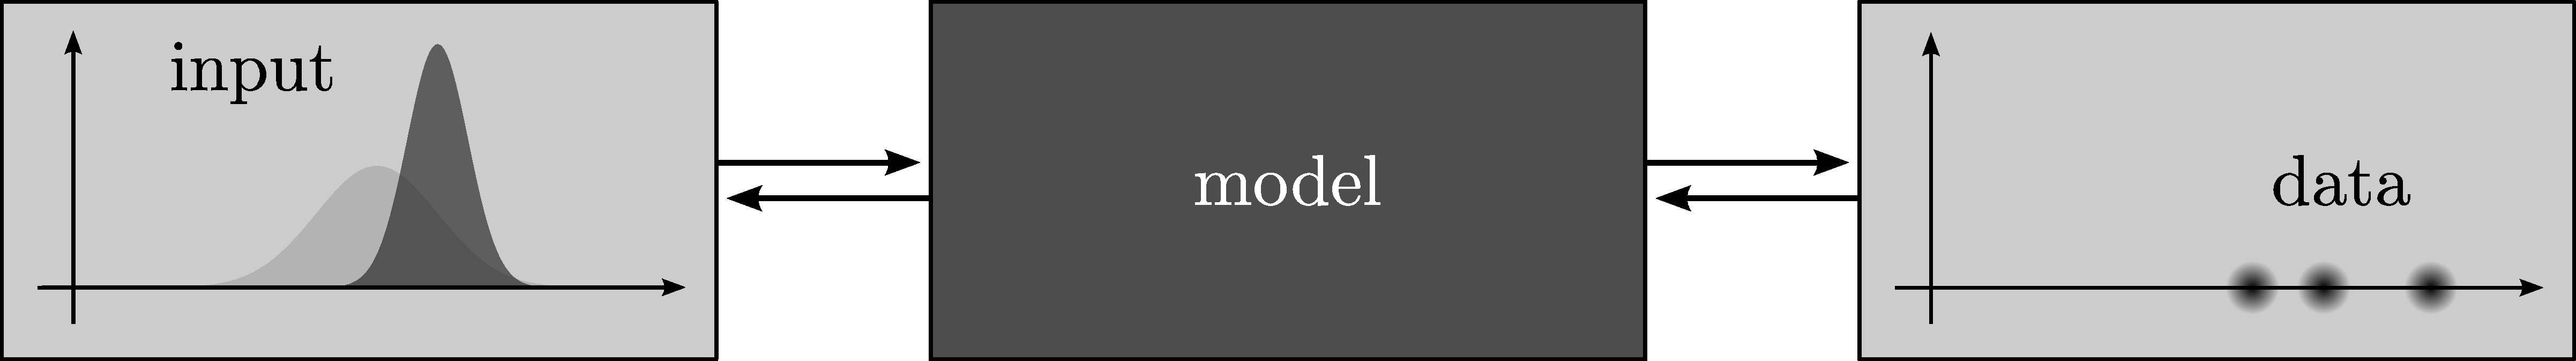
\includegraphics[width=13cm]{fig_Bayesian_InversePropagation}
  \caption[Inverse uncertainty quantification]{Inverse uncertainty quantification.}
  \label{fig:Inversion:InversePropagation}
\end{figure}
\par % MODEL PREDICTIONS
After having established the posterior distribution of the unknown parameters one is typically interested in making predictions.
In a straightforward way, a point estimate \(\hat{\bm{x}}\) may be used in order to predict the system response
\(\tilde{\bm{y}}^\prime = \mathcal{M}(\hat{\bm{x}},\bm{d}^\prime)\) under untested conditions \(\bm{d}^\prime \in \mathds{R}^\dimControl\).
% POSTERIOR UNCERTAINTY PROPAGATION
Analogous to \cref{eq:UQ:OutputMean,eq:UQ:OutputVariance}, one may be also interested in the propagated posterior uncertainty, e.g.\ the mean response and the covariance matrix
\begin{gather}
  \mathds{E}[\mathcal{M}(\bm{X},\bm{d}^\prime) \cond \bm{y}]
  = \int\limits_{\mathds{R}^\dimParam} \mathcal{M}(\bm{x},\bm{d}^\prime) \, \pi(\bm{x} \cond \bm{y}) \, \mathrm{d} \bm{x}, \label{eq:Bayesian:OutputMean} \\
  \mathrm{Cov}[\mathcal{M}(\bm{X},\bm{d}^\prime) \cond \bm{y}] = \int\limits_{\mathds{R}^\dimParam}
  \left( \mathcal{M}(\bm{x},\bm{d}^\prime) - \mathds{E}[\mathcal{M}(\bm{X},\bm{d}^\prime) \cond \bm{y}] \right)^2 \pi(\bm{x} \cond \bm{y}) \, \mathrm{d} \bm{x}. \label{eq:Bayesian:OutputVariance}
\end{gather}
% POSTERIOR PREDICTIVE DISTRIBUTION
While \cref{eq:Bayesian:OutputMean,eq:Bayesian:OutputVariance} take account of the remaining parameter uncertainty, they leave the output and measurement errors aside.
Those are incorporated into the posterior predictive distribution
\begin{equation} \label{eq:Inversion:PredictiveDistribution}
  \pi(\bm{y}^\prime \cond \bm{y})
  = \int\limits_{\mathds{R}^\dimParam} \mathcal{N}(\bm{y}^\prime \cond \mathcal{M}(\bm{x},\bm{d}^\prime), \bm{\Sigma}^\prime) \, \pi(\bm{x} \cond \bm{y}) \, \mathrm{d} \bm{x}.
\end{equation}
New data \(\bm{y}^\prime\) can be predicted for various conditions \(\bm{d}^\prime\) and residual covariances \(\bm{\Sigma}^\prime\) this way.
Note that the independence of the errors
\(\pi(\bm{\varepsilon},\bm{\varepsilon}^\prime) = \mathcal{N}(\bm{\varepsilon} \cond \bm{0}, \bm{\Sigma}) \, \mathcal{N}(\bm{\varepsilon}^\prime \cond \bm{0}, \bm{\Sigma}^\prime)\)
is implicitly assumed in \cref{eq:Inversion:PredictiveDistribution}.

\subsection{Multiple experiments} \label{sec:Bayesian:InverseProblems:MultipleExperiments}
% MULTIPLE EXPERIMENS
Sometimes it is meaningful to consider a number of similar experiments.
Even though the vector notation employed thus far implicitly permits their analysis already to some degree,
e.g.\ see the matrix form of linear regression in the next section, it is revelatory to treat them in a more explicit fashion.
Let us assume that a number of \(n \in \mathds{N}_{>0}\) different experiments are conducted,
in each of which the collected data are explained with a vector-valued forward model as \(\bm{y}_j = \mathcal{M}(\bm{x},\bm{d}_j) + \bm{\varepsilon}_j\).
The unknowns \(\bm{x}\) are constant throughout the experiments, whereas the experimental conditions \(\bm{d}_j\)
and covariances \(\bm{\Sigma}_j\) may very well differ for \(j = 1,\ldots,n\).
Assuming that the data in each experiment are conditionally independent given the unknowns, one has the data model
\begin{equation} \label{eq:Inversion:MultipleExperiments}
  \bm{Y}_1,\ldots,\bm{Y}_n \cond \bm{x} \sim \prod\limits_{j=1}^n \mathcal{N}(\bm{y}_j \cond \mathcal{M}(\bm{x},\bm{d}_j),\bm{\Sigma}_j).
\end{equation}
% VECTOR NOTATION
In connection with various types of model prediction errors and uncertainties, some generalizations of the described setup are discussed in \cref{sec:Bayesian:InverseProblems:ModelUncertainties}.
Against this background, \cref{eq:Inversion:MultipleExperiments} is rewritten as
\begin{equation} \label{eq:Inversion:MultipleExperiments:Vectorized}
  \begin{pmatrix}
    \bm{Y}_1 \\
    \vdots \\
    \bm{Y}_n \\
  \end{pmatrix}
  \cond \bm{x}
  \sim \mathcal{N} \left(
  \begin{pmatrix}
    \bm{y}_1 \\
    \vdots \\
    \bm{y}_n \\
  \end{pmatrix}
  \cond
  \begin{pmatrix}
    \mathcal{M}(\bm{x},\bm{d}_1) \\
    \vdots \\
    \mathcal{M}(\bm{x},\bm{d}_n) \\
  \end{pmatrix},
  \begin{pmatrix}
    \bm{\Sigma}_1 & \ldots & \bm{0}_{\dimData \times \dimData} \\
    \vdots & \ddots & \vdots \\
    \bm{0}_{\dimData \times \dimData} & \ldots & \bm{\Sigma}_n \\
  \end{pmatrix}
  \right).
\end{equation}
% LIKELIHOOD & POSTERIOR
For the corresponding likelihood function one has \(\mathcal{L}(\bm{x}) = \prod_{j=1}^n \mathcal{N}(\bm{y}_j \cond \mathcal{M}(\bm{x},\bm{d}_j),\bm{\Sigma}_j)\).
The Bayesian update to the posterior density \(\pi(\bm{x} \cond \bm{y}_1,\ldots,\bm{y}_n) \propto \mathcal{L}(\bm{x}) \pi(\bm{x})\) and all further analyses proceed as normal.

\subsection{Linear regression} \label{sec:Bayesian:InverseProblems:LinearRegression}
% LINEAR REGRESSION
In order to get a feel for inverse problems as discussed previously, we consider Bayesian linear regression.
This can be viewed as the prototype of a linear inverse problem and often has a simple solution, i.e.\ when the prior and the likelihood are conjugate to each other.
Details can be found in many references for Bayesian inference \cite{Bayesian:OHagan1994,Bayesian:Hoff2009} and regression analysis \cite{Statistics:Seber2003,Statistics:Yan2009}.
Following a discussion of the linear model with known error variance, the natural extension with an unknown variance is investigated.

\subsubsection{Known variance}
% LINEAR MODEL
In linear regression, the measured variables \(\tilde{\bm{y}} \in \mathds{R}^\dimData\) are linearly dependent on a vector of unknown coefficients \(\bm{x} \in \mathds{R}^\dimParam\).
The predictor-dependent design matrix \(\bm{A} \in \mathds{R}^{\dimData \times \dimParam}\) establishes this relation through \(\tilde{\bm{y}} = \bm{A} \bm{x}\).
A general linear regression model of the form as in \cref{eq:Inversion:NoisyData} is thus written as
\begin{equation} \label{eq:Linear:NoisyData}
  \bm{y} = \bm{A} \bm{x} + \bm{\varepsilon}.
\end{equation}
% ERROR MODEL
The actual observations \(\bm{y}\) are represented as a noisy version of the model outputs.
As in \cref{eq:Inversion:ErrorModel}, the noise is often modeled with a Gaussian distribution.
We consider spherical errors with a diagonal covariance matrix of the form \(\bm{\Sigma} = \sigma^2 \bm{I}_\dimData\),
where \(\bm{I}_\dimData\) is the \(\dimData \times \dimData\) identity matrix.
They are jointly distributed according to
\begin{equation} \label{eq:Linear:ErrorModel}
  \pi(\bm{\varepsilon}) = \mathcal{N}(\bm{\varepsilon} \cond \bm{0}, \sigma^2 \bm{I}_\dimData).
\end{equation}
% DATA MODEL
The probabilistic data model as in \cref{eq:Inversion:DataModel} is thus given as \(\bm{Y} \cond \bm{x} \sim \mathcal{N}(\bm{y} \cond \bm{A} \bm{x}, \sigma^2 \bm{I}_\dimData)\)
and the likelihood function in \cref{eq:Inversion:LikelihoodFunction} follows as \(\mathcal{L}(\bm{x}) = \mathcal{N}(\bm{y} \cond \bm{A} \bm{x}, \sigma^2 \bm{I}_\dimData)\).
\par % PRIOR DISTRIBUTION
As for the prior, one imposes a Gaussian distribution with a mean vector \(\bm{\mu}_0\) and a covariance matrix \(\bm{\Sigma}_0\) on the regressors.
This is done by setting
\begin{equation} \label{eq:Linear:PriorDensity}
  \pi(\bm{x}) = \mathcal{N}(\bm{x} \cond \bm{\mu}_0, \bm{\Sigma}_0).
\end{equation}
Again, the unknowns and the errors are treated as independent from one another.
% POSTERIOR DISTRIBUTION
Given the linear-normal model in \cref{eq:Linear:NoisyData,eq:Linear:ErrorModel,eq:Linear:PriorDensity},
one can easily show that the posterior \(\pi(\bm{x} \cond \bm{y}) \propto \mathcal{L}(\bm{x}) \pi(\bm{x})\) of the regression coefficients is the normal distribution
\begin{equation} \label{eq:Linear:PosteriorDensity}
  \pi(\bm{x} \cond \bm{y}) = \mathcal{N}(\bm{x} \cond \bm{\mu}_1, \bm{\Sigma}_1), \quad \text{with} \;\,
  \left\{
  \begin{aligned}
    \bm{\Sigma}_1 &= \left( \bm{\Sigma}_0^{-1} + \sigma^{-2} \bm{A}^\top \bm{A} \right)^{-1}, \\
    \bm{\mu}_1 &= \bm{\Sigma}_1 \left( \bm{\Sigma}_0^{-1} \bm{\mu}_0 + \sigma^{-2} \bm{A}^\top \bm{y} \right).
  \end{aligned}
  \right.
\end{equation}
\par % INTUITION
Some useful intuition about the problem can be obtained from \cref{eq:Linear:PosteriorDensity}.
On the one hand, in the limit of vanishing prior knowledge, i.e.\ \(\bm{\Sigma}_0^{-1}\) can be neglected,
the classical results \(\bm{\mu}_1 = (\bm{A}^\top \bm{A})^{-1} \bm{A}^\top \bm{y}\) and \(\bm{\Sigma}_1 = \sigma^2 (\bm{A}^\top \bm{A})^{-1}\) are obtained.
On the other hand, for \(\sigma^2 \rightarrow \infty\) one simply has \(\bm{\mu}_1 = \bm{\mu}_0\) and \(\bm{\Sigma}_1 = \bm{\Sigma}_0\), i.e.\ the prior knowledge dominates.

\subsubsection{Unknown variance}
% UNKNOWN VARIANCE
A straightforward extension to the linear regression model with known variance is based on the inference of the error variance as an additional unknown.
One considers an error model \(\pi(\bm{\varepsilon} \cond \sigma^2) = \mathcal{N}(\bm{\varepsilon} \cond \bm{0}, \sigma^2 \bm{I}_\dimData)\)
with a covariance matrix of the form \(\bm{\Sigma} = \sigma^2 \bm{I}_\dimData\).
The errors for different response variables are uncorrelated and share the same variance just as in \cref{eq:Linear:ErrorModel}.
Unlike before, however, the variance \(\sigma^2\) is now treated as uncertain and associated with a prior distribution \(\pi(\sigma^2)\).
The latter forms a marginal of the joint prior \(\pi(\bm{x},\sigma^2)\) which is not necessarily the product \(\pi(\bm{x},\sigma^2) = \pi(\bm{x}) \pi(\sigma^2)\).
A statistical model \(\bm{Y} \cond \bm{x},\sigma^2 \sim \mathcal{N}(\bm{y} \cond \bm{A} \bm{x}, \sigma^2 \bm{I}_\dimData)\)
gives rise to the likelihood function \(\mathcal{L}(\bm{x},\sigma^2) = \mathcal{N}(\bm{y} \cond \bm{A} \bm{x}, \sigma^2 \bm{I}_\dimData)\).
The posterior \(\pi(\bm{x},\sigma^2 \cond \bm{y}) \propto \mathcal{L}(\bm{x},\sigma^2) \pi(\bm{x},\sigma^2)\)
is then taken as the basis for the identification of the unknowns \((\bm{x},\sigma^2)\).
One may extract \(\pi(\bm{x} \cond \bm{y})\) and \(\pi(\sigma^2 \cond \bm{y})\) from the posterior by an appropriate marginalization as in \cref{eq:Bayesian:PosteriorMarginal}.
Before this formulation is simplified by using a conjugate prior for the variance \(\sigma^2\),
it is remarked that one may just as well assign a prior to the unknown standard deviation \(\sigma\).
See \cref{sec:Bayesian:ModelParametrization} for a discussion on related parametrization issues.
\par % PRIOR DISTRIBUTION
Similar to the precursory model with known variance, Bayesian linear regression with unknown variance possesses an explicit posterior presentation under a certain prior distribution.
This conjugate prior has the hierarchical structure \(\pi(\bm{x},\sigma^2) = \pi(\bm{x} \cond \sigma^2) \pi(\sigma^2)\).
The marginal prior of the variance \(\sigma^2 > 0\) is an inverse gamma distribution
\(\pi(\sigma^2) = \mathcal{IG}(\sigma^2 \cond \alpha_0,\beta_0) = \Gamma^{-1}(\alpha_0) \beta_0^{\alpha_0} (\sigma^2)^{-\alpha_0-1} \exp(-\beta_0/\sigma^2)\).
Here, \(\Gamma\) is the gamma function and \(\alpha_0,\beta_0 > 0\) are the shape and scale parameters of the distribution, respectively.
The conditional prior of the unknown coefficients \(\bm{x}\) is a normal distribution \(\pi(\bm{x} \cond \sigma^2) = \mathcal{N}(\bm{x} \cond \bm{\mu}_0, \sigma^2 \bm{\Sigma}_0)\)
with the mean \(\bm{\mu}_0\) and the \(\sigma^2\)-dependent covariance matrix \(\sigma^2 \bm{\Sigma}_0\).
All in all, the joint prior is the normal inverse gamma distribution
\begin{equation} \label{eq:Linear:UnknownSigmaPrior}
  \pi(\bm{x},\sigma^2)
  = \mathcal{N}(\bm{x} \cond \bm{\mu}_0, \sigma^2 \bm{\Sigma}_0) \, \mathcal{IG}(\sigma^2 \cond \alpha_0,\beta_0)
  = \mathcal{NIG}(\bm{x},\sigma^2 \cond \bm{\mu}_0,\bm{\Sigma}_0,\alpha_0,\beta_0).
\end{equation}
\par % POSTERIOR DISTRIBUTION
Given this prior, a straightforward calculation yields the posterior density \(\pi(\bm{x},\sigma^2 \cond \bm{y}) \propto \mathcal{L}(\bm{x},\sigma^2) \pi(\bm{x},\sigma^2)\) in a closed form.
In particular, the posterior can be analytically expressed as
\begin{equation} \label{eq:Linear:UnknownSigmaPosterior}
  \pi(\bm{x},\sigma^2 \cond \bm{y}) = \mathcal{NIG}(\bm{x},\sigma^2 \cond \bm{\mu}_1,\bm{\Sigma}_1,\alpha_1,\beta_1), \quad \text{with} \;\,
  \left\{
  \begin{aligned}
    \bm{\Sigma}_1 &= \left( \bm{\Sigma}_0^{-1} + \bm{A}^\top \bm{A} \right)^{-1}, \\
    \bm{\mu}_1 &= \bm{\Sigma}_1 \left( \bm{\Sigma}_0^{-1} \bm{\mu}_0 + \bm{A}^\top \bm{y} \right), \\
    \alpha_1 &= \alpha_0 + \frac{\dimData}{2}, \\
    \beta_1 &= \beta_0 + \frac{1}{2} \left( \bm{y}^\top \bm{y} + \bm{\mu}_0^\top \bm{\Sigma}_0 \bm{\mu}_0 - \bm{\mu}_1^\top \bm{\Sigma}_1 \bm{\mu}_1 \right).
  \end{aligned}
  \right.
\end{equation}
The posterior \(\pi(\bm{x},\sigma^2 \cond \bm{y}) = \pi(\bm{x} \cond \sigma^2,\bm{y}) \pi(\sigma^2 \cond \bm{y})
= \mathcal{N}(\bm{x} \cond \bm{\mu}_1, \sigma^2 \bm{\Sigma}_1) \, \mathcal{IG}(\sigma^2 \cond \alpha_1,\beta_1)\)
in \cref{eq:Linear:UnknownSigmaPosterior} is of the same normal inverse gamma shape as the prior in \cref{eq:Linear:UnknownSigmaPrior}.

\subsection{Model uncertainties} \label{sec:Bayesian:InverseProblems:ModelUncertainties}
% MODELING ERRORS
In many experimental situations, at least some of the simplifying assumptions made cannot actually be justified.
This concerns the idealizations formalized in \cref{eq:Inversion:NoisyData,eq:Inversion:ErrorModel,eq:Inversion:DataModel}.
While the inverse theory established so far focuses on epistemic parameter uncertainties, it woefully neglects various other forms of uncertainty.
The treatment of parametric variability is indeed the main topic of \cref{sec:PEM,sec:JRUES}.
Bayesian probability lends itself to an analysis of other sources of uncertainty and error, too.
A non-exhaustive synopsis of related methods is provided below.
They are based on a refined representation and parametrization of the relation between forward model predictions and real measurement data.
\par % ERROR MODELS
There is indeed a plethora of methods for representing and handling error or uncertainty in the context of predictive modeling.
This includes \emph{multiplicative errors} in the model outputs \(\bm{y} = \mathcal{M}(\bm{x},\bm{d}) \cdot (1 + \bm{\varepsilon})\)
and \emph{errors-in-variables}, i.e.\ the experimental conditions are only inexactly measured \cite{Uncertainty:Fuller1987,Uncertainty:Carroll2006,Uncertainty:Buonaccorsi2010}.
We do not further delve into these issues, but rather focus on additive measurement and modeling errors.

\subsubsection{Random error calibration}
% RESIDUAL CALIBRATION
It seems to be overly optimistic to start from the premise that the covariance matrix \(\bm{\Sigma}\) in \cref{eq:Inversion:ErrorModel} is prespecified before the data analysis.
In order to relax this limiting assumption, one can parametrize the error model conveniently
and infer its parameters as additional unknowns during data analysis \cite{Bayesian:Zhang2010,Bayesian:Zhang2011,Bayesian:Zhang2012}.
A simple example of this type of \emph{error calibration} was already encountered in \cref{sec:Bayesian:InverseProblems:LinearRegression}.
Let the error model \(\pi(\bm{\varepsilon} \cond \bm{\theta}) = \mathcal{N}(\bm{\varepsilon} \cond \bm{0}, \bm{\Sigma}(\bm{\theta}))\)
be parametrized by a possibly multivariate parameter vector \(\bm{\theta}\).
Note that this could encompass correlation parameters.
Eliciting a prior \(\pi(\bm{x},\bm{\theta})\) and constructing a likelihood \(\mathcal{L}(\bm{x},\bm{\theta}) = \mathcal{N}(\bm{y} - \mathcal{M}(\bm{x}) \cond \bm{0}, \bm{\Sigma}(\bm{\theta}))\)
allows for conditioning on the data via \(\pi(\bm{x},\bm{\theta} \cond \bm{y}) \propto \mathcal{L}(\bm{x},\bm{\theta}) \pi(\bm{x},\bm{\theta})\).
The way the likelihood is written signalizes that the formulation can be generalized beyond Gaussian errors.
A caveat is that the approach may require a fair bit of data, though.

\subsubsection{Predictive model correction}
% MODEL DISCREPANCY
While the error calibration as discussed above allows one to account for random sources of uncertainty, e.g.\ measurement noise,
it disregards systematic inadequacies of the forward model \cite{Bayesian:Ling2014,Bayesian:Sargsyan2015}.
The question of \emph{model discrepancy} is certainly tricky, though.
It concerns the model building process as a whole.
Let us consider an experimental scenario where the available predictive model shows considerable deficits but cannot be substituted with a better model.
Moreover, the data are too few to learn alternative predictive models, but they are still numerous enough to awaken the hope for an in-depth error analysis.
In this borderline situation, that lies exactly in between more model-centered uncertainty quantification and purely data-based machine learning,
one can try to detect and quantify the modeling errors by comparing the predicted system outputs to real data.
In turn, this can serve as a guide to model correction.
\par % MULTIPLE EXPERIMENTS
In the following, the multi-experiment setup from \cref{sec:Bayesian:InverseProblems:MultipleExperiments} is generalized in order to account for model discrepancy.
As a first step, the discrepancy is either treated as an unknown constant or a random variable.
In the next step, it is formulated as an unknown or even random function of the experimental conditions.
Some of the mathematical details are omitted for the sake of readability.
This concerns a few standard independence assumptions and the subtleties of certain basis representations.
\par % UNKNOWN CONSTANT
To begin with, the simplest extension is grounded on thinking of the model discrepancy as an unknown constant \(\bm{\delta} \in \mathds{R}^\dimData\).
Accordingly, for \(j=1,\ldots,n\) the actual measurements are represented as the sum \(\bm{y}_j = \mathcal{M}(\bm{x},\bm{d}_j) + \bm{\delta} + \bm{\varepsilon}_j\)
of the forward model response, the unknown offset and the random errors.
It is remarked that the unknown \(\bm{\delta}\) is fixed throughout all experiments.
The data are then probabilistically described by
\begin{equation} \label{eq:Inversion:Model:UnknownConstantDiscrepancy}
  \bm{Y}_1,\ldots,\bm{Y}_n \cond \bm{x},\bm{\delta} \sim \prod\limits_{j=1}^n \mathcal{N}(\bm{y}_j \cond \mathcal{M}(\bm{x},\bm{d}_j) + \bm{\delta}, \bm{\Sigma}_j).
\end{equation}
The corresponding likelihood function \(\mathcal{L}(\bm{x},\bm{\delta})\) follows easily.
One proceeds by imposing a prior \(\pi(\bm{x},\bm{\delta}) = \pi(\bm{x}) \pi(\bm{\delta})\) and learns the unknowns \((\bm{x},\bm{\delta})\)
via the Bayesian update \(\pi(\bm{x},\bm{\delta} \cond \bm{y}_1,\ldots,\bm{y}_n) \propto \mathcal{L}(\bm{x},\bm{\delta}) \pi(\bm{x},\bm{\delta})\).
Statistical identifiability or the lack thereof could be relevant issues at that.
\par % RANDOM VARIABLES
Another representation of model error in various experiments is a number of random variables
\(\bm{\Delta}_j \sim \mathcal{N}(\bm{\delta}_j \cond \bm{\mu}_{\bm{\Delta}},\bm{\Sigma}_{\bm{\Delta}})\).
For a clear exposition, these variables are assumed to be Gaussian with unknown mean \(\bm{\mu}_{\bm{\Delta}}\) and known covariance \(\bm{\Sigma}_{\bm{\Delta}}\).
They take on different values \(\bm{\Delta}_j = \bm{\delta}_j\) in each experiment.
Accordingly, the data are represented as \(\bm{y}_j = \mathcal{M}(\bm{x},\bm{d}_j) + \bm{\delta}_j + \bm{\varepsilon}_j\).
The discrepancy term now randomly varies across the experiments.
Conditionally on the unknowns \((\bm{x},\bm{\mu}_{\bm{\Delta}})\), the data are the sum of independent Gaussian variables and follow
\begin{equation} \label{eq:Inversion:Model:RandomVariableDiscrepancy}
  \bm{Y}_1,\ldots,\bm{Y}_n \cond \bm{x},\bm{\mu}_{\bm{\Delta}}
  \sim \prod\limits_{j=1}^n \mathcal{N}(\bm{y}_j \cond \mathcal{M}(\bm{x},\bm{d}_j)+ \bm{\mu}_{\bm{\Delta}}, \bm{\Sigma}_j + \bm{\Sigma}_{\bm{\Delta}}).
\end{equation}
Inference of the unknowns proceeds as for the related model in \cref{eq:Inversion:Model:UnknownConstantDiscrepancy}.
The likelihood function \(\mathcal{L}(\bm{x},\bm{\mu}_{\bm{\Delta}})\) results from \cref{eq:Inversion:Model:RandomVariableDiscrepancy}
and the joint prior is specified as \(\pi(\bm{x},\bm{\mu}_{\bm{\Delta}}) = \pi(\bm{x}) \pi(\bm{\mu}_{\bm{\Delta}})\).
Hence, the posterior is  \(\pi(\bm{x},\bm{\mu}_{\bm{\Delta}} \cond \bm{y}_1,\ldots,\bm{y}_n) \propto \mathcal{L}(\bm{x},\bm{\mu}_{\bm{\Delta}}) \pi(\bm{x},\bm{\mu}_{\bm{\Delta}})\).
Note that the identification of the mean value \(\bm{\mu}_{\bm{\Delta}}\) typically requires more than just a single experiment.
\par % UNKNOWN FUNCTION
An advanced approach is to treat the systematic model discrepancy as an unknown function \(\delta: \mathds{R}^\dimControl \rightarrow \mathds{R}^\dimData\).
It represents the model bias \(\delta(\bm{d})\) as a function of the experimental conditions \(\bm{d} \in \mathds{R}^\dimControl\).
For this reason, the error in an experiment \(j \in \{1,\ldots,n\}\) is a fixed yet unknown value \(\delta(\bm{d}_j)\) rather than a random outcome.
The data are consequentially modeled as \(\bm{y}_j = \mathcal{M}(\bm{x},\bm{d}_j) + \delta(\bm{d}_j) + \bm{\varepsilon}_j\).
Here, the discrepancy term effectively absorbs the systematic error components of the model predictions such that zero-mean errors are justified.
The goal of the analysis is now to identify both the unknown model parameters as well as the discrepancy function.
A prior model of the unknown function that is sloppily denoted as \(\pi(\delta(\cdot))\) has to be established,
e.g.\ by using an appropriate basis representation \cite{Bayesian:Farajpour2013,Bayesian:He2016:a} with prior distributions for the unknown coefficients.
The likelihood function \(\mathcal{L}(\bm{x},\delta(\cdot))\) would rest on the statistical model
\begin{equation} \label{eq:Inversion:Model:UnknownFunctionDiscrepancy}
  \bm{Y}_1,\ldots,\bm{Y}_n \cond \bm{x},\delta(\cdot) \sim \prod\limits_{j=1}^n \mathcal{N}(\bm{y}_j \cond \mathcal{M}(\bm{x},\bm{d}_j) + \delta(\bm{d}_j), \bm{\Sigma}_j).
\end{equation}
A Bayesian analysis then informs about the unknowns \((\bm{x},\delta(\cdot))\).
Letting \(\pi(\bm{x},\delta(\cdot)) = \pi(\bm{x}) \pi(\delta(\cdot))\) the posterior is
\(\pi(\bm{x},\delta(\cdot) \cond \bm{y}_1,\ldots,\bm{y}_n) \propto \mathcal{L}(\bm{x},\delta(\cdot)) \pi(\bm{x},\delta(\cdot))\).
After the calibration, one can eventually use the corrected model predictions \(\tilde{\bm{y}}^\prime = \mathcal{M}(\hat{\bm{x}},\bm{d}^\prime) + \hat{\delta}(\bm{d}^\prime)\)
in the interpolation regime, i.e.\ within the range of tested experimental conditions.
The extrapolation beyond this range requires a good deal of courage and caution, though.
Notice that the forward model \(\mathcal{M}(\bm{x},\bm{d})\) is not corrected as a function of the unknowns \(\bm{x}\), which are fixed across the experiments.
The model correction \(\delta(\bm{d})\) rather relates to \(\mathcal{M}(\bm{x},\bm{d})\) as a function of the covariates \(\bm{d}\), while the parameter \(\bm{x}\) attains its most plausible value.
Bear in mind that data must be collected for various different experimental conditions in order to meaningfully characterize the structural error.
\par % RANDOM FUNCTION
One could treat model discrepancy also as a random function, e.g.\ as an unknown realization of a stochastic process with priorly unknown hyperparameters.
In an original formulation \cite{Bayesian:Kennedy2001,Kriging:Higdon2004,Kriging:Higdon2015} and its multivariate generalizations \cite{Bayesian:Higdon2008:a,Bayesian:Higdon2008:b}
both the simulator \(\mathcal{M}(\bm{x},\bm{d})\) and the discrepancy function \(\delta(\bm{d})\) are nonparametrically represented as realizations of Gaussian processes.
At the same time it is conditioned on the observational data and the experimental design.
The hyperparameters of the mean \(m \colon \mathds{R}^\dimControl \rightarrow \mathds{R}^\dimData\) and the covariance function
\(c \colon \mathds{R}^\dimControl \times \mathds{R}^\dimControl \rightarrow \mathds{R}^{\dimData \times \dimData}\) are unknown themselves and therefore endowed with priors.
In a rather vague manner this is hinted at by writing \(\pi(m(\cdot))\) and \(\pi(c(\cdot,\cdot))\).
Given the unknowns \((\bm{x},m(\cdot),c(\cdot,\cdot))\), finite collections of random variables are jointly normal under the aforementioned modeling assumptions.
So are the data
\begin{equation} \label{eq:Inversion:Model:RandomFunctionDiscrepancy}
  \begin{aligned}
    \begin{pmatrix}
      \bm{Y}_1 \\
      \vdots \\
      \bm{Y}_n \\
    \end{pmatrix} \cond \bm{x},m(\cdot),c(\cdot,\cdot) \sim \mathcal{N}
    \left( \vphantom{\begin{pmatrix} \bm{y}_1 \\ \vdots \\ \bm{y}_n \end{pmatrix}} \!\! \right.
    \begin{pmatrix}
      \bm{y}_1 \\
      \vdots \\
      \bm{y}_n \\
    \end{pmatrix}
    \cond
    &\begin{pmatrix}
      \mathcal{M}(\bm{x},\bm{d}_1) \\
      \vdots \\
      \mathcal{M}(\bm{x},\bm{d}_n) \\
    \end{pmatrix}
    +
    \begin{pmatrix}
      m(\bm{d}_1)\\
      \vdots \\
      m(\bm{d}_n) \\
    \end{pmatrix}
    , \\
    &\begin{pmatrix}
      \bm{\Sigma}_1 + c(\bm{d}_1,\bm{d}_1) & \ldots & c(\bm{d}_1,\bm{d}_n) \\
      \vdots & \ddots & \vdots \\
       c(\bm{d}_n,\bm{d}_1) & \ldots & \bm{\Sigma}_n + c(\bm{d}_n,\bm{d}_n) \\
    \end{pmatrix}
    \left. \vphantom{\begin{pmatrix} \bm{y}_1 \\ \vdots \\ \bm{y}_n \end{pmatrix}} \!\! \right).
  \end{aligned}
\end{equation}
This can be compared to \cref{eq:Inversion:MultipleExperiments:Vectorized,eq:Inversion:Model:UnknownFunctionDiscrepancy}.
With the likelihood function \(\mathcal{L}(\bm{x},m(\cdot),c(\cdot,\cdot))\) that arises from \cref{eq:Inversion:Model:RandomFunctionDiscrepancy}
and the prior distribution \(\pi(\bm{x},m(\cdot),c(\cdot,\cdot)) = \pi(\bm{x}) \pi(m(\cdot)) \pi(c(\cdot,\cdot))\) one can construct the posterior
\(\pi(\bm{x},m(\cdot),c(\cdot,\cdot) \cond \bm{y}_1,\ldots,\bm{y}_n) \propto \mathcal{L}(\bm{x},m(\cdot),c(\cdot,\cdot)) \pi(\bm{x},m(\cdot),c(\cdot,\cdot))\).
The obtained results can be subsequently used for correcting model predictions and quantifying their uncertainty.
This is elegant in theory and important in practice \cite{Bayesian:Brynjarsdottir2014}.
It allows for Bayesian model validation \cite{Bayesian:Bayarri2007,Bayesian:Wang2009} and for a coherent management of the uncertainties
emerging from measurement errors, model inadequacies and a limited number of simulator runs \cite{Kriging:Bilionis2014}.
On the downside, the approach is quite complex and identifiability may very well become a problem \cite{Bayesian:Arendt2012:a,Bayesian:Arendt2012:b}.
Sufficiently numerous data subject to different experimental conditions have to be available.

\subsubsection{Model class comparison}
% MODEL UNCERTAINTY
After the consideration of the uncertainties and discrepancies of a single predictive model, one can also assess the relative plausibilities of multiple alternative models.
The evidence framework of \cref{sec:Bayesian:ModelEvidence} is eminently suitable for this kind of job.
A number \(L \in \mathds{N}_{>1} \) of different Bayesian models \(\bm{\mathcal{H}} = \{\mathcal{H}_1,\ldots,\mathcal{H}_L\}\) is considered.
They are referred to as \emph{model classes} in common parlance.
Each \(\mathcal{H} \in \bm{\mathcal{H}}\) is characterized by a forward model \(\mathcal{M}_{\mathcal{H}}\)
with \(\dimControl_{\mathcal{H}} \in \mathds{N}_{>0}\) control variables \(\bm{d}_{\mathcal{H}} \in \mathds{R}^{\dimControl_{\mathcal{H}}}\)
and \(\dimParam_{\mathcal{H}} \in \mathds{N}_{>0}\) unknown parameters \(\bm{x}_{\mathcal{H}} \in \mathds{R}^{\dimParam_{\mathcal{H}}}\),
a prior distribution \(\pi(\bm{x}_{\mathcal{H}} \cond \mathcal{H})\) and an error model \(\pi(\bm{\varepsilon}_{\mathcal{H}} \cond \bm{\theta}_{\mathcal{H}},\mathcal{H})\).
The latter depends on model-specific parameters \(\bm{\theta}_{\mathcal{H}}\) and might be associated with a prior \(\pi(\bm{\theta}_{\mathcal{H}} \cond \mathcal{H})\).
% MODEL EVIDENCE
The plausibilities of different model classes can then be assessed by reference to their model evidences \(\scale_{\mathcal{H}}\) in \cref{eq:Bayesian:ModelLikelihood}.
More generally, when a model prior \(\pi(\mathcal{H})\) is available, the model posterior distribution \(\pi(\mathcal{H} \cond \bm{y}) \propto \scale_{\mathcal{H}} \pi(\mathcal{H})\)
in \cref{eq:Bayesian:ModelPosterior} provides the basis for data-informed model class comparison, selection and averaging.
\par % ENGINEERING APPLICATIONS
In inverse modeling, the outlined way of evaluating model classes can be deployed for comparing and selecting forward models \cite{Bayesian:Mthembu2011,Bayesian:Riley2011,Bayesian:Riley2014}.
Averaging over the model classes quantifies the prediction uncertainty in this context \cite{Bayesian:Park2010,Bayesian:Park2011}.
It is worth noting that random error models can undergo the same procedure, too.
For instance, one might be interested in different error correlation structures \cite{Bayesian:Simoen2013:a}.